
%(BEGIN_QUESTION)
% Copyright 2010, Tony R. Kuphaldt, released under the Creative Commons Attribution License (v 1.0)
% This means you may do almost anything with this work of mine, so long as you give me proper credit

The following circuit senses temperature using a thermistor with a positive temperature coefficient (i.e. resistance increases as temperature increases):

$$\includegraphics[width=15.5cm]{i02924x01.eps}$$

First, determine the voltage we should read at the voltmeter with the thermistor at or near room temperature.  

Next, identify the likelihood of each specified fault for this circuit, supposing the voltmeter registers 0 volts with the thermistor at room temperature, and a voltage measurement taken between terminals D and F registers 10 volts.  Consider each fault one at a time (i.e. no coincidental faults), determining whether or not each fault could independently account for {\it all} measurements and symptoms in this circuit.

% No blank lines allowed between lines of an \halign structure!
% I use comments (%) instead, so that TeX doesn't choke.

$$\vbox{\offinterlineskip
\halign{\strut
\vrule \quad\hfil # \ \hfil & 
\vrule \quad\hfil # \ \hfil & 
\vrule \quad\hfil # \ \hfil \vrule \cr
\noalign{\hrule}
%
% First row
{\bf Fault} & {\bf Possible} & {\bf Impossible} \cr
%
\noalign{\hrule}
%
% Another row
Thermistor failed open &  &  \cr
%
\noalign{\hrule}
%
% Another row
Fixed resistor failed open &  &  \cr
%
\noalign{\hrule}
%
% Another row
Wire A-D failed open &  &  \cr
%
\noalign{\hrule}
%
% Another row
Wire F-J failed open &  &  \cr
%
\noalign{\hrule}
%
% Another row
Wire E-H failed open &  &  \cr
%
\noalign{\hrule}
%
% Another row
Thermistor failed shorted &  &  \cr
%
\noalign{\hrule}
%
% Another row
Fixed resistor failed shorted &  &  \cr
%
\noalign{\hrule}
%
% Another row
Short between terminals G-H &  &  \cr
%
\noalign{\hrule}
%
% Another row
Short between terminals E-F &  &  \cr
%
\noalign{\hrule}
%
% Another row
Short between terminals D-E &  &  \cr
%
\noalign{\hrule}
} % End of \halign 
}$$ % End of \vbox


\vfil 

\underbar{file i02924}
\eject
%(END_QUESTION)





%(BEGIN_ANSWER)

This is a graded question -- no answers or hints given!

%(END_ANSWER)





%(BEGIN_NOTES)

Voltage at room temperature should be half the supply voltage: {\bf 5 volts DC}, because the thermistor is supposed to exhibit a resistance of 1000 ohms at room temperature.  With the thermistor at 1 k$\Omega$ and the fixed-value resistor measuring the same, a 1:2 voltage divider is formed which will take the 10 volt supply voltage and divide it in half.

\vskip 10pt

With the voltmeter registering 0 volts, we know there is either a short-circuit in parallel with the meter (ensuring equipotentiality and therefore 0 voltage drop) or there is an open circuit fault somewhere that severs the connection between the voltmeter and the power source:

% No blank lines allowed between lines of an \halign structure!
% I use comments (%) instead, so that TeX doesn't choke.

$$\vbox{\offinterlineskip
\halign{\strut
\vrule \quad\hfil # \ \hfil & 
\vrule \quad\hfil # \ \hfil & 
\vrule \quad\hfil # \ \hfil \vrule \cr
\noalign{\hrule}
%
% First row
{\bf Fault} & {\bf Possible} & {\bf Impossible} \cr
%
\noalign{\hrule}
%
% Another row
Thermistor failed open &  & $\surd$ \cr
%
\noalign{\hrule}
%
% Another row
Fixed resistor failed open & $\surd$ &  \cr
%
\noalign{\hrule}
%
% Another row
Wire A-D failed open & $\surd$ &  \cr
%
\noalign{\hrule}
%
% Another row
Wire F-J failed open &  & $\surd$ \cr
%
\noalign{\hrule}
%
% Another row
Wire E-H failed open & $\surd$ &  \cr
%
\noalign{\hrule}
%
% Another row
Thermistor failed shorted & $\surd$ &  \cr
%
\noalign{\hrule}
%
% Another row
Fixed resistor failed shorted &  & $\surd$ \cr
%
\noalign{\hrule}
%
% Another row
Short between terminals G-H &  & $\surd$ \cr
%
\noalign{\hrule}
%
% Another row
Short between terminals E-F & $\surd$ &  \cr
%
\noalign{\hrule}
%
% Another row
Short between terminals D-E &  & $\surd$ \cr
%
\noalign{\hrule}
} % End of \halign 
}$$ % End of \vbox



%INDEX% Troubleshooting review: electric circuits

%(END_NOTES)


